\newpage
\chapter{Mappings and Sets}
Leave this page blank Intentionally.
\chapter{Logic and Proofs}
\section{Personal Practice}
\begin{bt} \end{bt}
\begin{bt} \end{bt}
\begin{bt} \end{bt}
\begin{bt} \end{bt}
\begin{bt} \end{bt}
\begin{bt} \end{bt}
\begin{bt} \end{bt}
\begin{bt} \end{bt}
\begin{bt} \end{bt}
\begin{bt} \end{bt}
\begin{bt} \end{bt}
\begin{bt} \end{bt}
\begin{bt} \end{bt}
\begin{bt} \end{bt}
\begin{bt} \end{bt}
\begin{bt} \end{bt}
\begin{bt} \end{bt}
\begin{bt} \end{bt}
\begin{bt} \end{bt}
\begin{bt} \end{bt}
\begin{bt} \end{bt}
\begin{bt} \end{bt}
\begin{bt} \end{bt}
\begin{bt} \end{bt}
\begin{bt} \end{bt}
\begin{bt} \end{bt}
\begin{bt} \end{bt}
\begin{bt} \end{bt}
\begin{longfbox}
    \begin{bt} \label{pro:practice2.29}
        Verify that the given argument form is valid
        \begin{enumerate}
            \item[] $\forall x \in \mathcal U: p(x) \rightarrow q(x)$
            \item[] $a \in \mathcal U$
            \item[] $\neg q(a)$
            \item[] $\therefore \neg p(a)$
        \end{enumerate}
    \end{bt}
\end{longfbox}

Solution:
\begin{table}[hbt!]
    \centering
    \begin{tabular}{|l | l|} 
    \hline
    Statement forms & Justification\\ [0.5ex] 
    \hline
        1. $\forall x \in \mathcal U: p(x) \rightarrow q(x)$ & Given \\
        2. $\forall x \in \mathcal U: \neg q(x) \rightarrow \neg p(x)$ & Equivalent form of (1) \\
        3. Let $a \in \mathcal U$ the arbitrary & Given assumption \\
        4. $\therefore \neg q(a) \rightarrow \neg p(a)$ & (2),(3) Principle of Generalization \\
        5. $\neg q(a)$ & Given \\
        6. $\therefore \neg p(a)$ & Valid because of (4), (5) \\
    \hline
    \end{tabular}
\end{table} 

\newpage
\begin{longfbox}
    \begin{bt} \label{pro:practice2.30}
        Verify that the given argument form is valid
        \begin{enumerate}
            \item[] $\forall x \in \mathcal U: p(x) \lor q(x)$
            \item[] $a \in \mathcal U$
            \item[] $\neg p(a)$
            \item[] $\therefore q(a)$
        \end{enumerate}
    \end{bt}
\end{longfbox}

Solution
\begin{table}[hbt!]
    \centering
    \begin{tabular}{|l | l|} 
    \hline
    Statement forms & Justification\\ [0.5ex] 
    \hline
        1. $\forall x \in \mathcal U: p(x) \lor q(x)$ & Given \\
        2. $\forall x \in \mathcal U: \neg p(x) \lor q(x)$ & Equivalent form of (1) \\
        3. $a \in \mathcal U$ & Given \\
        4. $\neg p(a) \lor q(a)$ & (2), (3) Principle of Specification \\
        5. $\therefore \neg p(a)$ & Valid bacause of (3), (4) \\
    \hline
    \end{tabular}
\end{table}

\begin{longfbox}
    \begin{bt} \label{pro:practice2.31}
        Verify that the given argument form is valid
        \begin{enumerate}
            \item[] $\forall x \in \mathcal U: p(x) \lor q(x)$
            \item[] $\forall x \in \mathcal U: \neg q(x)$
            \item[] $\therefore \forall x \in \mathcal U: \neg p(x)$
        \end{enumerate}
    \end{bt}
\end{longfbox}

Solution
\begin{table}[hbt!]
    \centering
    \begin{tabular}{|l | l|} 
    \hline
    Statement forms & Justification\\ [0.5ex] 
    \hline
        1. $\forall x \in \mathcal U: p(x) \rightarrow q(x)$ & Given \\
        2. $\forall x \in \mathcal U: \neg q(x) \rightarrow \neg p(x)$ & Equivalent form of (1) \\
        3. $\forall x \in \mathcal U: q(x)$ & Given \\
        4. $\therefore \neg p(x)$ & Valid because of (2), (4) \\
    \hline
    \end{tabular}
\end{table}

\begin{longfbox}
    \begin{bt} \label{pro:practice2.32}
        Verify that the given argument form is valid
        \begin{enumerate}
            \item[] $\forall x \in \mathcal U: p(x) \lor q(x)$
            \item[] $\forall x \in \mathcal U: \neg p(x)$
            \item[] $\therefore \forall x \in \mathcal U: q(x)$
        \end{enumerate}
    \end{bt}
\end{longfbox}

Solution
\begin{table}[hbt!]
    \centering
    \begin{tabular}{|l | l|} 
    \hline
    Statement forms & Justification\\ [0.5ex] 
    \hline
        1. $\forall x \in \mathcal U: p(x) \lor q(x)$ & Given \\
        2. $\forall x \in \mathcal U: \neg p(x) \lor q(x)$ & Equivalent form of (1) \\
        3. $\forall x \in \mathcal U: \neg p(x)$ & Given \\
        4. $\therefore \forall x \in \mathcal U: \neg q(x)$ & Valid bacause of (2), (3) \\
    \hline
    \end{tabular}
\end{table}

\newpage
\begin{longfbox}
    \begin{bt} \label{pro:practice2.33}
        Verify that the given argument form is valid
        \begin{enumerate}
            \item[] $\forall x \in \mathcal U: p(x)$
            \item[] $\forall x \in \mathcal U: q(x)$
            \item[] $a \in \mathcal U$
            \item[] $\therefore p(a) \land q(a)$
        \end{enumerate}
    \end{bt}
\end{longfbox}

Solution
\begin{table}[hbt!]
    \centering
    \begin{tabular}{|l | l|} 
    \hline
    Statement forms & Justification\\ [0.5ex] 
    \hline
        1. $\forall x \in \mathcal U: p(x)$ & Given \\
        2. $\forall x \in \mathcal U: q(x)$ & Given \\
        3. $\forall x \in \mathcal U: p(x) \land q(x)$ & (1), (2) Principle of Conjunction \\
        4. $a \in \mathcal U$ & Given \\
        5. $\therefore p(a) \land q(a)$ & (3), (4) Principle of Specification \\
    \hline
    \end{tabular}
\end{table}

\begin{longfbox}
    \begin{bt} \label{pro:practice2.34}
        Verify that the given argument form is valid
        \begin{enumerate}
            \item[] $\forall x \in \mathcal U: p(x) \rightarrow q(s)$
            \item[] $\forall x \in \mathcal U: q(x) \rightarrow r(x)$
            \item[] $a \in \mathcal U$
            \item[] $\therefore p(a) \rightarrow r(a)$
        \end{enumerate}
    \end{bt}
\end{longfbox}

Solution
\begin{table}[hbt!]
    \centering
    \begin{tabular}{|l | l|} 
    \hline
    Statement forms & Justification\\ [0.5ex] 
    \hline
        1. $\forall x \in \mathcal U: p(x) \rightarrow q(s)$ & Given \\
        2. $\forall x \in \mathcal U: q(x) \rightarrow r(x)$ & Given \\
        3. $\forall x \in \mathcal U: p(x) \rightarrow r(x)$ & (1), (2) Transivity of $\rightarrow$ \\
        4. $a \in \mathcal U$ & Given \\
        5. $\therefore p(a) \rightarrow r(a)$ & (3), (4) Principle of Specification \\
    \hline
    \end{tabular}
\end{table}

\newpage
\begin{longfbox}
    \begin{bt} \label{pro:practice2.35}
        Verify that the given argument form is valid
        \begin{enumerate}
            \item[] $\forall x \in \mathcal U: p(x) \rightarrow q(s)$
            \item[] $\forall x \in \mathcal U: q(x) \rightarrow r(x)$
            \item[] $\therefore \forall x \in \mathcal U: p(x) \land r(x)$
        \end{enumerate}
    \end{bt}
\end{longfbox}

Solution
\begin{table}[hbt!]
    \centering
    \begin{tabular}{|l | l|}
    \hline
    Statement forms & Justification\\ [0.5ex]
    \hline
        1. $\forall x \in \mathcal U: p(x) \rightarrow q(s)$ & Given \\
        2. $\forall x \in \mathcal U: q(x) \rightarrow r(x)$ & Given \\
        3. $\therefore \forall x \in \mathcal U: p(x) \land r(x)$ & (1), (2) Principle of Conjunction \\
    \hline
    \end{tabular}
\end{table}

\begin{longfbox}
    \begin{bt} \label{pro:practice2.36}
        Verify that the given argument form is valid
        \begin{enumerate}
            \item[] $\forall x \in \mathcal U: p(x) \rightarrow q(s)$
            \item[] $\forall x \in \mathcal U: q(x) \rightarrow r(x)$
            \item[] $\therefore \forall x \in \mathcal U: p(x) \rightarrow r(x)$
        \end{enumerate}
    \end{bt}
\end{longfbox}

Solution
\begin{table}[hbt!]
    \centering
    \begin{tabular}{|l | l|}
    \hline
    Statement forms & Justification\\ [0.5ex]
    \hline
        1. $\forall x \in \mathcal U: p(x) \rightarrow q(s)$ & Given \\
        2. $\forall x \in \mathcal U: q(x) \rightarrow r(x)$ & Given \\
        3. $\therefore \forall x \in \mathcal U: p(x) \rightarrow r(x)$ & (1), (2) Transivity of $\rightarrow$ \\
    \hline
    \end{tabular}
\end{table}

\begin{longfbox}
    \begin{bt} \label{pro:practice2.37}
        Verify that the given argument form is valid
        \begin{enumerate}
            \item[] $\forall x \in \mathcal U: p(x) \lor q(x)$
            \item[] $a \in \mathcal U$
            \item[] $q(a) \rightarrow r(a)$
            \item[] $\therefore p(a) \lor r(a)$
        \end{enumerate}
    \end{bt}
\end{longfbox}

Solution
\begin{table}[hbt!]
    \centering
    \begin{tabular}{|l | l|}
    \hline
    Statement forms & Justification\\ [0.5ex]
    \hline
        1. $\forall x \in \mathcal U: p(x) \lor q(x)$ & Given \\
        2. $\forall x \in \mathcal U: \neg p(x) \rightarrow q(x)$ & Equivalent form of (1) \\
        3. $a \in \mathcal U$ & Given \\
        4. $\neg p(a) \rightarrow q(a)$ & (2), (3) Principle of Specification \\
        5. $q(a) \rightarrow r(a)$ & Given \\
        6. $\neg p(a) \rightarrow r(a)$ & (4), (5) Transivity of $\rightarrow$ \\
        6. $\therefore p(a) \lor r(a)$ & Equivalent form of (6) \\
    \hline
    \end{tabular}
\end{table}

\newpage
\begin{longfbox}
    \begin{bt} \label{pro:practice2.38}
        Verify that the given argument form is valid
        \begin{enumerate}
            \item[] $\forall x \in \mathcal U: p(x) \land \neg q(x)$
            \item[] $\forall x \in \mathcal U: q(x) \lor \neg r(x)$
            \item[] $\therefore \forall x \in \mathcal U: \neg p(x) \rightarrow r(x)$
        \end{enumerate}
    \end{bt}
\end{longfbox}

Solution
\begin{table}[hbt!]
    \centering
    \begin{tabular}{|l | l|}
    \hline
    Statement forms & Justification\\ [0.5ex]
    \hline
        1. $\forall x \in \mathcal U: p(x) \land \neg q(x)$ & Given \\
        2. $\forall x \in \mathcal U: p(x)$ & Principle of Simplification \\
        3. $\forall x \in \mathcal U: p(x) \lor r(x)$ & Principle of Addition \\
        4. $\therefore \forall x \in \mathcal U: \neg p(x) \rightarrow r(x)$ & Equivalent form of (3) \\
    \hline
    \end{tabular}
\end{table}

\begin{longfbox}
    \begin{bt} \label{pro:practice2.39}
        Verify that the given argument form is invalid
        \begin{enumerate}
            \item[] $\forall x \in \mathcal U: p(x) \lor q(x)$
            \item[] $\forall x \in \mathcal U: \neg p(x)$
            \item[] $\therefore \forall x \in \mathcal U: \neg q(x)$
        \end{enumerate}
    \end{bt}
\end{longfbox}
Solution
\begin{figure}[hbt!]
\centering
\begin{tikzpicture}[fill=gray]
      \draw ( 0,0 ) circle (2) (-0.5,1.2)  node [text=black,above] {$P$}
            ( 3,0 ) circle (2) (3.8,1.2)  node [text=black,above] {$Q$}
            (-3,-3) rectangle (8,4) node [text=black,above] {$\mathcal U$};
      \filldraw[black] (3,0) circle (2pt) node[anchor=west] {$b$};
\end{tikzpicture}
\caption{Venn diagram for problem 1.1.1 \\
      - P: is the set of $x$ satisfies $p(x)$.\\
      - Q: is the set of $x$ satisfies $q(x)$.\\
      - $\exists b\in\mathcal U: p(b)\lor q(b), \neg p(b), q(b)$ so given argument is invalid
}
\end{figure}

\begin{longfbox}
    \begin{bt} \label{pro:practice2.40}
        Verify that the given argument form is invalid
        \begin{enumerate}
            \item[] $\forall x \in \mathcal U: p(x) \lor q(x)$
            \item[] $\forall x \in \mathcal U: q(x) \lor r(x)$
            \item[] $\therefore \forall x \in \mathcal U: p(x) \lor r(x)$
        \end{enumerate}
    \end{bt}
\end{longfbox}
Solution
\begin{figure}[hbt!]
\centering
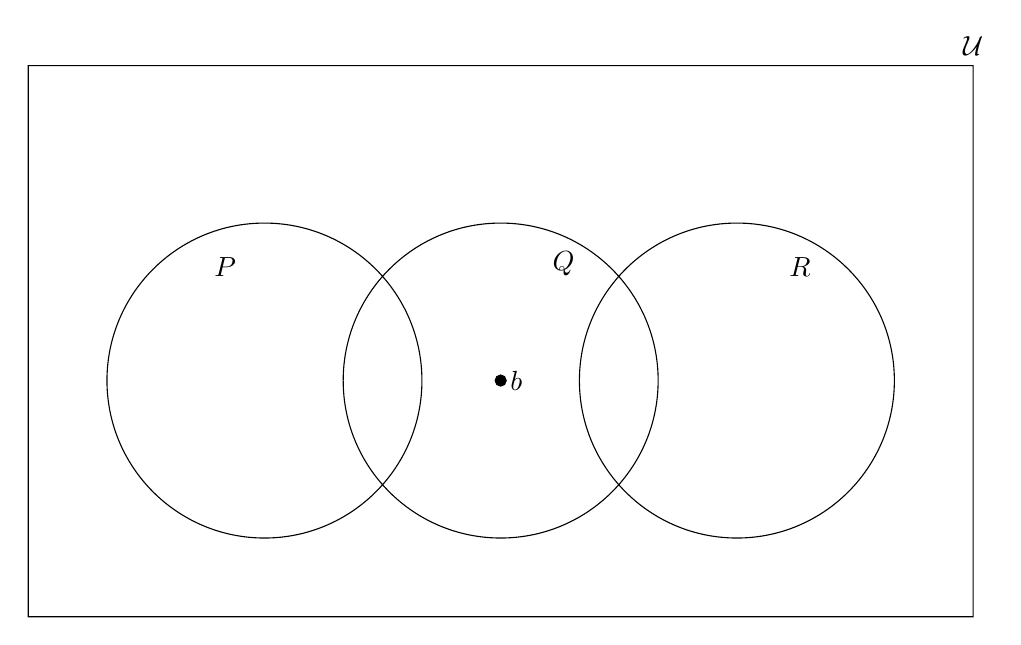
\begin{tikzpicture}[fill=gray]
      \draw ( 0,0 ) circle (2) (-0.5,1.2)  node [text=black,above] {$P$}
            ( 3,0 ) circle (2) (3.8,1.2)  node [text=black,above] {$Q$}
            ( 6,0 ) circle (2) (6.8,1.2)  node [text=black,above] {$R$}
            (-3,-3) rectangle (9,4) node [text=black,above] {$\mathcal U$};
      \filldraw[black] (3,0) circle (2pt) node[anchor=west] {$b$};
\end{tikzpicture}
\caption{Venn diagram for problem 1.1.1 \\
      - P: is the set of $x$ satisfies $p(x)$.\\
      - Q: is the set of $x$ satisfies $q(x)$.\\
      - R: is the set of $x$ satisfies $r(x)$.\\
      - $\exists b\in\mathcal U: p(b)\lor q(b), q(b)\lor r(b), \neg (p(b)\lor r(b))$ so given argument is invalid
}
\end{figure}

\newpage
\begin{longfbox}
    \begin{bt} \label{pro:practice2.41}
        Verify that the given argument form is invalid
        \begin{enumerate}
            \item[] $\forall x \in \mathcal U: p(x) \lor q(x)$
            \item[] $a \in \mathcal U$
            \item[] $p(a)\land q(a)$
            \item[] $\therefore \forall x \in \mathcal U: p(x) \land q(x)$
        \end{enumerate}
    \end{bt}
\end{longfbox}
Solution
\begin{figure}[hbt!]
\centering
\begin{tikzpicture}[fill=gray]
      \draw ( 0,0 ) circle (2) (-0.5,1.2)  node [text=black,above] {$P$}
            ( 3,0 ) circle (2) (3.8,1.2)  node [text=black,above] {$Q$}
            (-3,-3) rectangle (9,4) node [text=black,above] {$\mathcal U$};
      \filldraw[black] (1.3,0) circle (2pt) node[anchor=west] {$a$};
      \filldraw[black] (3,0) circle (2pt) node[anchor=west] {$b$};
\end{tikzpicture}
\caption{Venn diagram for problem 1.1.1 \\
      - P: is the set of $x$ satisfies $p(x)$.\\
      - Q: is the set of $x$ satisfies $q(x)$.\\
      - $a$ is the point satisfies $p(x) \land q(x)$.\\
      - $\exists b\in\mathcal U: \neg (p(b)\land q(b))$ so given argument is invalid
}
\end{figure}

\newpage
\begin{longfbox}
    \begin{bt} \label{pro:practice2.42}
        Verify that the given argument form is invalid
        \begin{enumerate}
            \item[] $\forall x \in \mathcal U: p(x) \rightarrow q(x)$
            \item[] $a \in \mathcal U$
            \item[] $q(a) \rightarrow p(a)$
            \item[] $\therefore \forall x \in \mathcal U: q(x) \rightarrow p(x)$
        \end{enumerate}
    \end{bt}
\end{longfbox}
Solution
\begin{figure}[hbt!]
\centering
\begin{tikzpicture}[fill=gray]
      \draw ( 0,0 ) circle (2) (-0.5,1.2)  node [text=black,above] {$P$}
            ( 3,0 ) circle (2) (3.8,1.2)  node [text=black,above] {$Q$}
            (-3,-3) rectangle (9,4) node [text=black,above] {$\mathcal U$};
      \filldraw[black] (1.3,0) circle (2pt) node[anchor=west] {$a$};
      \filldraw[black] (3,0) circle (2pt) node[anchor=west] {$b$};
\end{tikzpicture}
\caption{Venn diagram for problem 1.1.1 \\
      - P: is the set of $x$ satisfies $p(x)$.\\
      - Q: is the set of $x$ satisfies $q(x)$.\\
      - $\forall x \in \mathcal U: p(x)\rightarrow q(x) \equiv \neg p(x)\lor q(x)$ \\
      - $a \in \mathcal U$ is the point satisfies $q(a)\rightarrow p(a) \equiv \neg q(a)\lor p(a)$ \\
      - $\exists b\in\mathcal U: \neg(q(b)\rightarrow p(b)) \equiv \neg(q(b) \rightarrow p(b))$ so given argument is invalid
}
\end{figure}

\newpage
\begin{longfbox}
    \begin{bt} \label{pro:practice2.43}
        Test the validity of below arguments
    \end{bt}
\end{longfbox}
Solution:
\begin{enumerate}
    \item[(a)] Let: \\
        - $l$ is statement "London is in Denmark" \\
        - $p$ is statement "Paris is in French" \\
        Then we can present argument as:
        \begin{enumerate}
            \item[] $\neg l \rightarrow \neg p$
            \item[] $p$
            \item[] $\therefore l$
        \end{enumerate}
        Verify:
        \begin{table}[hbt!]
            \centering
            \begin{tabular}{|l | l|}
            \hline
            Statement forms & Justification\\ [0.5ex]
            \hline
                1. $\neg l \rightarrow \neg p$ & Given \\
                2. $p \rightarrow l$ & Equivalent form of (1) \\
                3. $p$ & Given \\
                4. $\therefore l$ & Modus Ponens (2), (3) \\
            \hline
            \end{tabular}
        \end{table}

    \item[(b)] Let: \\
        - $s$ is statement "study" \\
        - $f$ is statement "fail mathematics" \\
        Then we can present argument as:
        \begin{enumerate}
            \item[] $s \rightarrow \neg f$
            \item[] $\neg s$
            \item[] $\therefore f$
        \end{enumerate}
        In case: $s=F, f=F$, then $(s\rightarrow \neg f) \land \neg s= T = \neg f$ so above statement is invalid

    \newpage
    \item[(c)] Let: \\
        - $s$ is statement "6 is even" \\
        - $t$ is statement "2 devides 7" \\
        - $f$ is statement "5 is prime" \\
        Then we can present argument as:
        \begin{enumerate}
            \item[] $s \rightarrow \neg t$
            \item[] $\neg f \lor t$
            \item[] $f$
            \item[] $\therefore \neg s$
        \end{enumerate}
        Verify:
        \begin{table}[hbt!]
            \centering
            \begin{tabular}{|l | l|}
            \hline
            Statement forms & Justification\\ [0.5ex]
            \hline
                1. $s \rightarrow \neg t$ & Given \\
                2. $\neg f \lor t$ & Given \\
                3. $f \rightarrow t$ & Equivalent form of (2) \\
                4. $t \rightarrow \neg s$ & Equivalent form of (1) \\
                5. $f \rightarrow \neg s$ & Transivity of $\rightarrow$ from (3), (4) \\
                6. $f$ & Given \\
                7. $\therefore \neg s$ & Modus Ponens (5), (6) \\
            \hline
            \end{tabular}
        \end{table}

    \item[(d)] Let: \\
        - $b$ is statement "It is wife's birthday" \\
        - $f$ is statement "I bring flowers" \\
        - $w$ is statement "I work late" \\
        - $f$ is statement "5 is prime" \\
        Then we can present argument as:
        \begin{enumerate}
            \item[] $b \land f$
            \item[] $b \lor w$
            \item[] $\neg f$
            \item[] $\therefore w$
        \end{enumerate}
        In case $s=\mathbb{1}, f=\mathbb{1}, w=\mathbb{1}$ \\
        then $b\land f = \mathbb{1}, b\lor w = \mathbb{1}$ \\
        then $(b\land f) \land (b\lor w) \land \neg f = \mathbb{0} \neq w$ so above statement is invalid
    
    \newpage
    \item[(e)] Let: \\
        - $w$ is statement "I work" \\
        - $s$ is statement "I study" \\
        - $p$ is statement "I pass mathematics" \\
        Then we can present argument as:
        \begin{enumerate}
            \item[] $w \rightarrow \neg s$
            \item[] $w \lor p$
            \item[] $p$
            \item[] $\therefore s$
        \end{enumerate}
        In case $w=\mathbb{0}, p=\mathbb{0}, s=\mathbb{1}$ \\
        then $w\rightarrow \neg s = \mathbb{1}, w\lor p = \mathbb{0}$ \\
        then $w(\rightarrow \neg s) \land (w\lor p) \land p = \mathbb{0} \neq s$ so above statement is invalid
    
    \item[(f)] Let: \\
        - $w$ is statement "I work" \\
        - $s$ is statement "I study" \\
        - $p$ is statement "I pass mathematics" \\
        Then we can present argument as:
        \begin{enumerate}
            \item[] $w \rightarrow \neg s$
            \item[] $w \lor p$
            \item[] $w$
            \item[] $\therefore p$
        \end{enumerate}
        In case $w=\mathbb{1}, p=\mathbb{1}, s=\mathbb{1}$ \\
        then $w\rightarrow \neg s = \mathbb{0}, w\lor p = \mathbb{1}$ \\
        then $w(\rightarrow \neg s) \land (w\lor p) \land w = \mathbb{0} \neq p$ so above statement is invalid
\end{enumerate}

\newpage
\begin{longfbox}
    \begin{bt} \label{pro:practice2.44}
        Prove below statement by induction
    \end{bt}
\end{longfbox}
Solution:
\begin{enumerate}
    \item[(a)] $\forall n\geq 0: \displaystyle\sum^{n}_{i=1} i = \frac{n(n+1)}{2}$ \\
        Verify given equation in case $n=0$:
            \begin{align}
                \displaystyle\sum^{0}_{i=1} i &= \frac{0(0+1)}{2} = 0 \label{eqn:1}
            \end{align}
        Verify given equation in case $n=1$:
            \begin{align}
                \displaystyle\sum^{1}_{i=1} i &= \frac{1(1+1)}{2} = 1 \label{eqn:2}
            \end{align}
        Induction: Assume that above statement is correct with an arbitrary $k \geq 0$, then\\
        \begin{align}
            \displaystyle\sum^{k+1}_{i=1} i &= \displaystyle\sum^{k}_{i=1} i + (k+1) \\
                                            &= \frac{k(k+1)}{2} + (k+1) \\
                                            &= \frac{(k+1)((k+1)+1)}{2} \label{eqn:3}
        \end{align}
        From \ref{eqn:1}, \ref{eqn:2} and \ref{eqn:3}, the statement is proved
    
    \item[(b)] $\forall n\geq 0: \displaystyle\sum^{n}_{i=1} i^2 = \frac{n(n+1)(2n+1)}{6}$ \\
        Verify given equation in case $n=0$:
            \begin{align}
                \displaystyle\sum^{0}_{i=1} i^2 &= \frac{0(0+1)(2*0+1)}{6} = 0 \label{eqn:4}
            \end{align}
        Verify given equation in case $n=1$:
            \begin{align}
                \displaystyle\sum^{1}_{i=1} i^2 &= \frac{1(1+1)(2+1)}{6} = 1 \label{eqn:5}
            \end{align}
        Induction: Assume that above statement is correct with an arbitrary $k \geq 0$, then\\
        \begin{align}
            \displaystyle\sum^{k+1}_{i=1} i^2 &= \displaystyle\sum^{k}_{i=1} i^2 + (k+1)^2 \\
                                            &= \frac{k(k+1)(2k+1)}{6} + (k+1)^2 \\
                                            &= \frac{(k+1)((k+1)+1)(2(k+1)+1)}{6} \label{eqn:6}
        \end{align}
        From \ref{eqn:4}, \ref{eqn:5} and \ref{eqn:6}, the statement is proved
    
    \newpage
    \item[(c)] $\forall n\geq 0: \displaystyle\sum^{n}_{i=1} i^3 = \frac{n^2(n+1)^2}{4}$ \\
        Verify given equation in case $n=0$:
            \begin{align}
                \displaystyle\sum^{0}_{i=1} i^3 &= \frac{0^2(0+1)^2}{4} = 0 \label{eqn:7}
            \end{align}
        Verify given equation in case $n=1$:
            \begin{align}
                \displaystyle\sum^{1}_{i=1} i^3 &= \frac{1^2(1+1)^2}{4} = 1 \label{eqn:8}
            \end{align}
        Induction: Assume that above statement is correct with an arbitrary $k \geq 0$, then\\
        \begin{align}
            \displaystyle\sum^{k+1}_{i=1} i^3 &= \displaystyle\sum^{k}_{i=1} i^3 + (k+1)^3 \\
                                            &= \frac{k^2(k+1)^2}{4} + (k+1)^3 \\
                                            &= \frac{(k+1)^2((k+1)+1)^2}{4} \label{eqn:9}
        \end{align}
        From \ref{eqn:7}, \ref{eqn:8} and \ref{eqn:9}, the statement is proved
    
    \item[(d)] $\forall n\geq 0: \displaystyle\sum^{n}_{i=1} (2i+1)^2 = \frac{(n+1)(2n+1)(2n+3)}{3}$ \\
        Verify given equation in case $n=0$:
            \begin{align}
                \displaystyle\sum^{0}_{i=0} (2i+1)^2 &= \frac{(0+1)(2*0+1)(2*0+3)}{3} = 1 \label{eqn:10}
            \end{align}
        Verify given equation in case $n=1$:
            \begin{align}
                \displaystyle\sum^{1}_{i=0} (2i+1)^2 &= \frac{(1+1)(2*1+1)(2*1+3)}{3} = 10 \label{eqn:11}
            \end{align}
        Induction: Assume that above statement is correct with an arbitrary $k \geq 0$, then\\
        \begin{align}
            \displaystyle\sum^{k+1}_{i=0} (2i+1)^2 &= \displaystyle\sum^{k}_{i=0} (2i+1)^2 + (2(k+1)+1)^2 \\
                                            &= \frac{(k+1)(2k+1)(2k+3)}{3} + (2k+3)^2 \\
                                            &= \frac{((k+1)+1)(2(k+1)+1)(2(k+1)+3)}{3} \label{eqn:12}
        \end{align}
        From \ref{eqn:10}, \ref{eqn:11} and \ref{eqn:12}, the statement is proved

    \newpage
    \item[(e)] $\forall n\geq 0: \displaystyle\sum^{n}_{i=1} i(i+1) = \frac{n(n+1)(n+2)}{3}$ \\
        Verify given equation in case $n=0$:
            \begin{align}
                \displaystyle\sum^{0}_{i=1} i(i+1) &= \frac{0(0+1)(0+2)}{3} = 0 \label{eqn:13}
            \end{align}
        Verify given equation in case $n=1$:
            \begin{align}
                \displaystyle\sum^{1}_{i=1} i(i+1) &= \frac{1(1+1)(1+2)}{3} = 2 \label{eqn:14}
            \end{align}
        Induction: Assume that above statement is correct with an arbitrary $k \geq 0$, then\\
        \begin{align}
            \displaystyle\sum^{k+1}_{i=1} i(i+1) &= \displaystyle\sum^{k}_{i=1} i(i+1) + (k+1)((k+1)+1) \\
                                            &= \frac{k(k+1)(k+2)}{3} + (k+1)(k+2) \\
                                            &= \frac{(k+1)((k+1)+1)((k+1)+2)}{3} \label{eqn:15}
        \end{align}
        From \ref{eqn:13}, \ref{eqn:14} and \ref{eqn:15}, the statement is proved
    
    \item[(f)] $\forall n\geq 0: \displaystyle\sum^{n}_{i=1} i(i+1)(i+2) = \frac{n(n+1)(n+2)(n+3)}{4}$ \\
        Verify given equation in case $n=0$:
            \begin{align}
                \displaystyle\sum^{0}_{i=1} i(i+1)(i+2) &= \frac{0(0+1)(0+2)(0+3)}{4} = 0 \label{eqn:16}
            \end{align}
        Verify given equation in case $n=1$:
            \begin{align}
                \displaystyle\sum^{1}_{i=1} i(i+1)(i+2) &= \frac{1(1+1)(1+2)(1+3)}{4} = 6 \label{eqn:17}
            \end{align}
        Induction: Assume that above statement is correct with an arbitrary $k \geq 0$, then\\
        \begin{align}
            \displaystyle\sum^{k+1}_{i=1} i(i+1)(i+2) &= \displaystyle\sum^{k}_{i=1} i(i+1)(i+2) + (k+1)(k+2)(k+3) \\
                                            &= \frac{k(k+1)(k+2)(k+3)}{4} + (k+1)(k+2)(k+3) \\
                                            &= \frac{(k+1)(k+2)(k+3)(k+4)}{4} \label{eqn:18}
        \end{align}
        From \ref{eqn:16}, \ref{eqn:17} and \ref{eqn:18}, the statement is proved
    
    \newpage
    \item[(g)] $\forall n\geq 0: \displaystyle\sum^{n}_{i=1} ii! = (n+1)!-1$ \\
        Verify given equation in case $n=0$:
            \begin{align}
                \displaystyle\sum^{0}_{i=1} ii! &= (0+1)!-1 = 0 \label{eqn:19}
            \end{align}
        Verify given equation in case $n=1$:
            \begin{align}
                \displaystyle\sum^{1}_{i=1} ii! &= (1+1)!-1 = 1 \label{eqn:20}
            \end{align}
        Induction: Assume that above statement is correct with an arbitrary $k \geq 0$, then\\
        \begin{align}
            \displaystyle\sum^{k+1}_{i=1} ii! &= \displaystyle\sum^{k}_{i=1} ii! + (k+1)(k+1)! \\
                                            &= (k+1)!-1 + (k+1)(k+1)! \\
                                            &= (k+1)! + (k+1)!(k+1) -1 \\
                                            &= (k+2)! - 1 \label{eqn:21}
        \end{align}
        From \ref{eqn:19}, \ref{eqn:20} and \ref{eqn:21}, the statement is proved
    
    \item[(h)] $\forall n\geq 1: \displaystyle\sum^{n}_{i=1} \frac{1}{i(i+1)} = \frac{n}{n+1}$ \\
    Verify given equation in case $n=1$:
        \begin{align}
            \displaystyle\sum^{1}_{i=1} \frac{1}{i(i+1)} &= \frac{1}{1+1} = \frac{1}{2} \label{eqn:23}
        \end{align}
    Verify given equation in case $n=2$:
        \begin{align}
            \displaystyle\sum^{2}_{i=1} \frac{1}{i(i+1)} &= \frac{2}{2+1} = \frac{2}{3} \label{eqn:23}
        \end{align}
    Induction: Assume that above statement is correct with an arbitrary $k \geq 0$, then\\
    \begin{align}
        \displaystyle\sum^{k+1}_{i=1} \frac{1}{i(i+1)} &= \displaystyle\sum^{k}_{i=1} \frac{1}{i(i+1)} + \frac{1}{(k+1)(k+2)} \\
                                        &= \frac{k}{k+1} + \frac{1}{(k+1)(k+2)} \\
                                        &= \frac{k(k+2)}{(k+1)(k+2)} + \frac{1}{(k+1)(k+2)} \\
                                        &= \frac{(k+1)^2}{(k+1)(k+2)} \\
                                        &= \frac{k+1}{k+1+1} \label{eqn:24}
    \end{align}
    From \ref{eqn:22}, \ref{eqn:23} and \ref{eqn:24}, the statement is proved
    
    \newpage
    \item[(i)] $\forall n\geq 0: \displaystyle\sum^{n}_{i=1} i2^i = (n-1)2^{n+1}+2$ \\
    Verify given equation in case $n=0$:
        \begin{align}
            \displaystyle\sum^{0}_{i=1} i2^i &= (0-1)2^{0+1}+2 = 0 \label{eqn:25}
        \end{align}
    Verify given equation in case $n=1$:
        \begin{align}
            \displaystyle\sum^{1}_{i=1} i2^i &= (1-1)2^{1+1}+2 = 2 \label{eqn:26}
        \end{align}
    Induction: Assume that above statement is correct with an arbitrary $k \geq 0$, then\\
    \begin{align}
        \displaystyle\sum^{k+1}_{i=1} i2^i &= \displaystyle\sum^{k}_{i=1} i2^i + (k+1)2^{k+1} \\
                                        &= (k-1)2^{k+1} +2 + (k+1)2^{k+1} \\
                                        &= 2k2^{k+1} + 2 \\
                                        &= (k+1-1)2^{k+1+1} +2 \label{eqn:27}
    \end{align}
    From \ref{eqn:25}, \ref{eqn:26} and \ref{eqn:27}, the statement is proved
    
    \item[(j)] $\forall n\geq 0, a\neq 1: \displaystyle\sum^{n}_{i=1} ia^i = \frac{na^{n+2}-(n+1)a^{n+1}+a}{(a-1)^2}$ \\
    Verify given equation in case $n=0$:
        \begin{align}
            \displaystyle\sum^{0}_{i=1} ia^i &= \frac{0a^{0+2}-(0+1)a^{0+1}+a}{(a-1)^2} = 0 \label{eqn:28}
        \end{align}
    Verify given equation in case $n=1$:
        \begin{align}
            \displaystyle\sum^{1}_{i=1} ia^i &= \frac{1a^{1+2}-(1+1)a^{1+1}+a}{(a-1)^2} = a \label{eqn:29}
        \end{align}
    Induction: Assume that above statement is correct with an arbitrary $k \geq 0$, then\\
    \begin{align}
        \displaystyle\sum^{k+1}_{i=1} ia^i &= \displaystyle\sum^{k}_{i=1} ia^i + (k+1)a^{k+1} \\
                                        &= \frac{ka^{k+2}-(k+1)a^{k+1}+a}{(a-1)^2} + (k+1)a^{k+1} \\
                                        &= \frac{(k+1)a^{k+1+2}-(k+1+1)a^{k+1+1}+a}{(a-1)^2} \label{eqn:30}
    \end{align}
    From \ref{eqn:28}, \ref{eqn:29} and \ref{eqn:30}, the statement is proved
    
    \newpage
    \item[(k)] $\forall n\geq 0: \displaystyle\sum^{n}_{i=1} i^22^i = n^22^{n+1}-n2^{n+2}+3.2^{n+1}-6$ \\
    Verify given equation in case $n=0$:
        \begin{align}
            \displaystyle\sum^{0}_{i=1} i^22^i &= 0^22^{0+1}-0.2^{0+2}+3.2^{0+1}-6 = 0 \label{eqn:31}
        \end{align}
    Verify given equation in case $n=1$:
        \begin{align}
            \displaystyle\sum^{1}_{i=1} i^22^i &= 1^22^{1+1}-1.2^{1+2}+3.2^{1+1}-6 = 2 \label{eqn:32}
        \end{align}
    Induction: Assume that above statement is correct with an arbitrary $k \geq 0$, then\\
    \begin{align}
        \displaystyle\sum^{k+1}_{i=1} i^22^i &= \displaystyle\sum^{k}_{i=1} i^22^i + (k+1)^22^{k+1} \\
                                        &= k^22^{k+1}-k2^{k+2}+3.2^{k+1}-6 + (k+1)^22^{k+1} \\
                                        &= (k+1)^22^{k+1+1}-(k+1)2^{k+1+2}+3.2^{k+1+1}-6 \label{eqn:33}
    \end{align}
    From \ref{eqn:31}, \ref{eqn:32} and \ref{eqn:33}, the statement is proved
    
    \item[(l)] $\forall n\geq 0: \displaystyle\sum^{n}_{i=1} i^22^{n-i} = 2^{n+3}-2^{n+1}-n^2-4n-6$ \\
    Verify given equation in case $n=0$:
        \begin{align}
            \displaystyle\sum^{0}_{i=1} i^22^{n-i} &= 2^{0+3}-2^{0+1}-0^2-4.0-6 = 0 \label{eqn:34}
        \end{align}
    Verify given equation in case $n=1$:
        \begin{align}
            \displaystyle\sum^{1}_{i=1} i^22^{n-i} &= 2^{1+3}-2^{1+1}-1^2-4.1-6 = 1 \label{eqn:35}
        \end{align}
    Induction: Assume that above statement is correct with an arbitrary $k \geq 0$, then\\
    \begin{align}
        \displaystyle\sum^{k+1}_{i=1} i^22^{n-i} &= \displaystyle\sum^{k}_{i=1} i^22^{n-i} + (k+1)^22^{n-i} \\
                                        &= 2^{k+3}-2^{k+1}-k^2-4k-6 + (k+1)^22^{k+1} \\
                                        &= 2^{k+1+3}-2^{k+1+1}-(k+1)^2-4(k+1)-6 \label{eqn:36}
    \end{align}
    From \ref{eqn:34}, \ref{eqn:35} and \ref{eqn:36}, the statement is proved
    
    \newpage
    \item[(m)] $\forall n\geq 0: \displaystyle\sum^{n}_{i=1} \frac{1}{n+i} = \displaystyle\sum^{n}_{i=1} (\frac{1}{2i-1}-\frac{1}{2i})$ \\
    First of all, just consider these examples:
        \begin{enumerate}
            \item [i)] $n=0$
                \begin{align}
                    \displaystyle\sum^{0}_{i=1} \frac{1}{0+i} = 0 \label{eqn:37}
                \end{align}
            \item [ii)] $n=1$
                \begin{align}
                    \displaystyle\sum^{1}_{i=1} \frac{1}{1+i} = \frac{1}{2} \label{eqn:38}
                \end{align}
            \item [iii)] $n=2$
                \begin{align}
                    \displaystyle\sum^{2}_{i=1} \frac{1}{2+i} =\ 
                    \frac{1}{3}+\frac{1}{4} =\ 
                    \displaystyle\sum^{1}_{i=1} \frac{1}{1+i} -\frac{1}{2}+\frac{1}{3}+\frac{1}{4} \label{eqn:39}
                \end{align}
            \item [iv)] $n=3$
                \begin{align}
                    \displaystyle\sum^{3}_{i=1} \frac{1}{3+i} =\
                    \frac{1}{4}+\frac{1}{5} +\frac{1}{6} =\ 
                    \displaystyle\sum^{2}_{i=1} \frac{1}{2+i} -\frac{1}{3}+\frac{1}{5}+\frac{1}{6} \label{eqn:40}
                \end{align}
            \item[v)] ... (so on)
        \end{enumerate}
    From \ref{eqn:37}, \ref{eqn:38}, \ref{eqn:39} and \ref{eqn:40}. We can present like this:
    \begin{align}
        \forall n\geq 2: \displaystyle\sum^{k+1}_{i=1} \frac{1}{k+1+i} =\
        \displaystyle\sum^{k}_{i=1} \frac{1}{k+i} -\frac{1}{k+1}+\frac{1}{2k+1}+\frac{1}{2k+2} \label{eqn:40}
    \end{align}
    Verify given equation in case $n=0$:
        \begin{align}
            \displaystyle\sum^{0}_{i=1} \frac{1}{0+i} &= \displaystyle\sum^{0}_{i=1} (\frac{1}{2i-1}-\frac{1}{2i}) = 0 \label{eqn:41}
        \end{align}
    Verify given equation in case $n=1$:
        \begin{align}
            \displaystyle\sum^{1}_{i=1} \frac{1}{1+i} &= \displaystyle\sum^{1}_{i=1} (\frac{1}{2i-1}-\frac{1}{2i}) = \frac{1}{2.1-1}-\frac{1}{2.1} = \frac{1}{2} \label{eqn:42}
        \end{align}
    Verify given equation in case $n=2$:
        \begin{align}
            \displaystyle\sum^{2}_{i=1} \frac{1}{2+i} &=\
            \displaystyle\sum^{2}_{i=1} (\frac{1}{2i-1}-\frac{1}{2i}) =\ 
            \frac{1}{2.1-1}-\frac{1}{2.1} + \frac{1}{2.2-1}-\frac{1}{2.2} = \frac{7}{12} \label{eqn:43}
        \end{align}
    
    Induction: Assume that above statement is correct with an arbitrary $k \geq 2$, and based on \ref{eqn:40}:\\
    \begin{align}
        \forall n\geq 2: \displaystyle\sum^{k+1}_{i=1} \frac{1}{k+1+i} &=\
        \displaystyle\sum^{k}_{i=1} \frac{1}{k+i} -\frac{1}{k+1}+\frac{1}{2k+1}+\frac{1}{2k+2} \\
        &= \displaystyle\sum^{k}_{i=1} (\frac{1}{2i-1}-\frac{1}{2i}) -\frac{1}{k+1}+\frac{1}{2k+1}+\frac{1}{2k+2} \\
        &= \displaystyle\sum^{k}_{i=1} (\frac{1}{2i-1}-\frac{1}{2i}) +\frac{1}{2k+1}+(\frac{1}{2k+2}-\frac{1}{k+1}) \\
        &= \displaystyle\sum^{k}_{i=1} (\frac{1}{2i-1}-\frac{1}{2i}) +(\frac{1}{2(k+1)-1}-\frac{1}{2(k+1)}) \\
        &= \displaystyle\sum^{k+1}_{i=1} (\frac{1}{2i-1}-\frac{1}{2i}) \label{eqn:44}
    \end{align}
    From \ref{eqn:41}, \ref{eqn:42}, \ref{eqn:43} and \ref{eqn:44}, the statement is proved

\end{enumerate}
